\documentclass{standalone}
\usepackage{tikz}
\usetikzlibrary{patterns, positioning}


\begin{document}
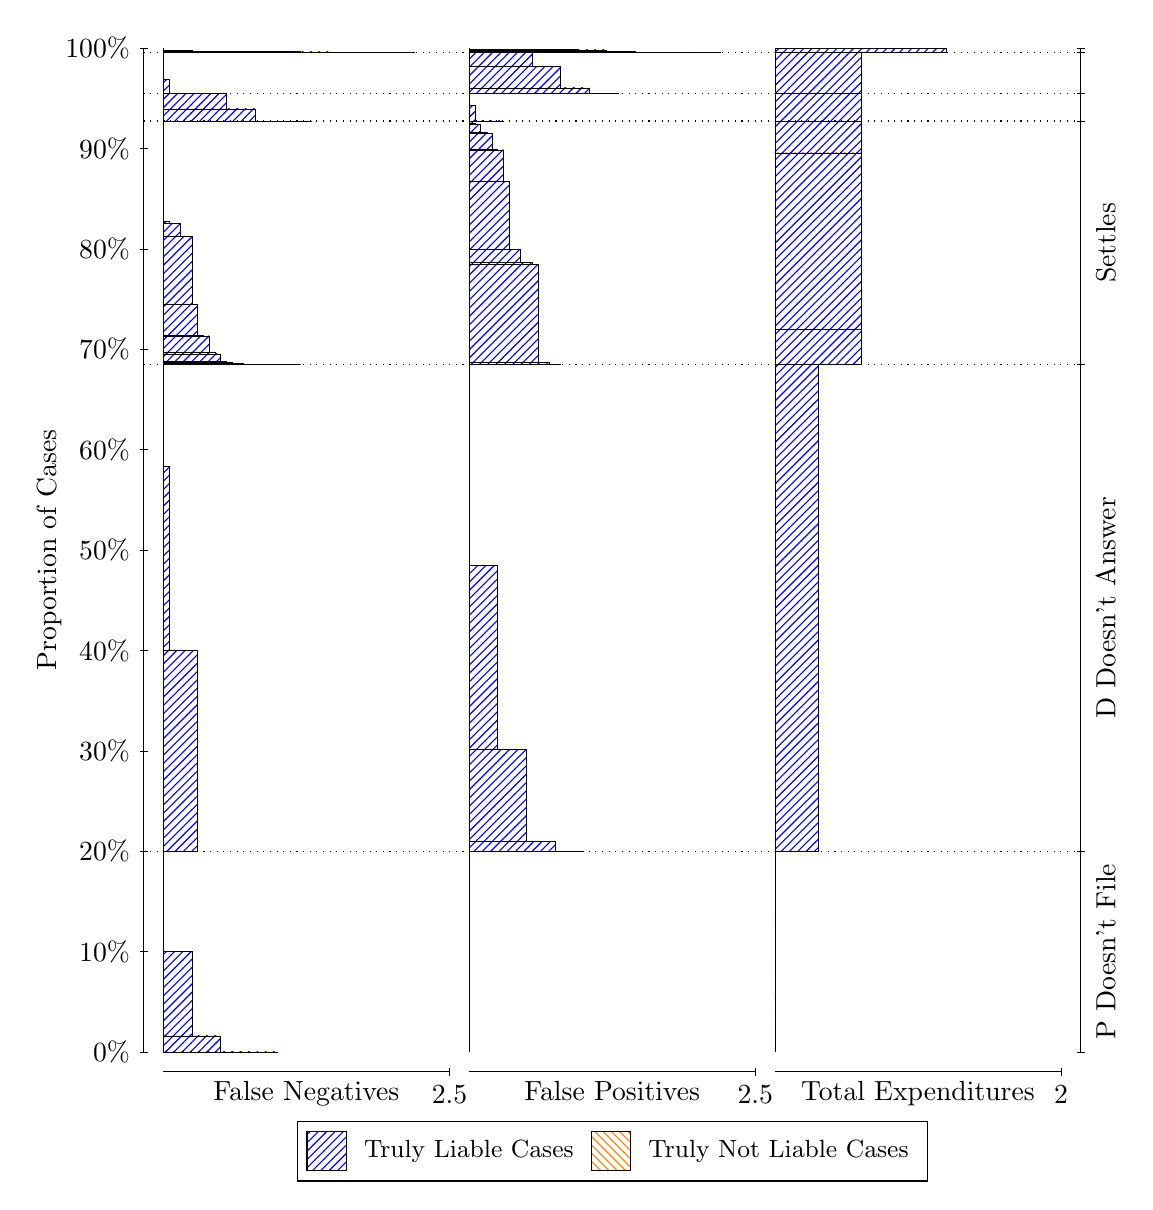
\begin{tikzpicture}
\draw[black, very thin] (1.5,1.75) -- (1.5,14.5);
\node[rotate=90, text=black, anchor=center] at (0.3, 8.125) {Proportion of Cases};
\draw[black, very thin] (1.45,1.75) -- (1.55,1.75);
\node[text=black, anchor=east] at (1.45, 1.75) {0\%};
\draw[black, very thin] (1.45,3.025) -- (1.55,3.025);
\node[text=black, anchor=east] at (1.45, 3.025) {10\%};
\draw[black, very thin] (1.45,4.3) -- (1.55,4.3);
\node[text=black, anchor=east] at (1.45, 4.3) {20\%};
\draw[black, very thin] (1.45,5.575) -- (1.55,5.575);
\node[text=black, anchor=east] at (1.45, 5.575) {30\%};
\draw[black, very thin] (1.45,6.85) -- (1.55,6.85);
\node[text=black, anchor=east] at (1.45, 6.85) {40\%};
\draw[black, very thin] (1.45,8.125) -- (1.55,8.125);
\node[text=black, anchor=east] at (1.45, 8.125) {50\%};
\draw[black, very thin] (1.45,9.4) -- (1.55,9.4);
\node[text=black, anchor=east] at (1.45, 9.4) {60\%};
\draw[black, very thin] (1.45,10.675) -- (1.55,10.675);
\node[text=black, anchor=east] at (1.45, 10.675) {70\%};
\draw[black, very thin] (1.45,11.95) -- (1.55,11.95);
\node[text=black, anchor=east] at (1.45, 11.95) {80\%};
\draw[black, very thin] (1.45,13.225) -- (1.55,13.225);
\node[text=black, anchor=east] at (1.45, 13.225) {90\%};
\draw[black, very thin] (1.45,14.5) -- (1.55,14.5);
\node[text=black, anchor=east] at (1.45, 14.5) {100\%};

\draw[black, very thin] (13.4,1.75) -- (13.4,14.5);
\draw[black, very thin] (13.35,1.75) -- (13.45,1.75);
\node[anchor=west] at (13.35, 1.75) {};
\draw[black, very thin] (13.35,4.2994) -- (13.45,4.2994);
\node[anchor=west] at (13.35, 4.2994) {};
\draw[black, very thin] (13.35,10.479) -- (13.45,10.479);
\node[anchor=west] at (13.35, 10.479) {};
\draw[black, very thin] (13.35,13.573) -- (13.45,13.573);
\node[anchor=west] at (13.35, 13.573) {};
\draw[black, very thin] (13.35,13.926) -- (13.45,13.926);
\node[anchor=west] at (13.35, 13.926) {};
\draw[black, very thin] (13.35,14.442) -- (13.45,14.442);
\node[anchor=west] at (13.35, 14.442) {};
\draw[black, very thin] (13.35,14.5) -- (13.45,14.5);
\node[anchor=west] at (13.35, 14.5) {};

\draw[black, very thin, pattern color=blue, pattern=north east lines] (1.75,1.75) rectangle (3.2033,1.75);
\draw[black, very thin, pattern color=blue, pattern=north east lines] (1.75,1.75) rectangle (2.84,1.7517);
\draw[black, very thin, pattern color=blue, pattern=north east lines] (1.75,1.7517) rectangle (2.4767,1.954);
\draw[black, very thin, pattern color=blue, pattern=north east lines] (1.75,1.954) rectangle (2.1133,3.0265);
\draw[black, very thin, pattern color=orange, pattern=north west lines] (1.75,3.0265) rectangle (1.75,3.0265);
\draw[black, very thin, pattern color=blue, pattern=north east lines] (1.75,3.0265) rectangle (1.75,4.2994);
\draw[black, very thin, pattern color=blue, pattern=north east lines] (1.75,4.2994) rectangle (2.186,6.8473);
\draw[black, very thin, pattern color=blue, pattern=north east lines] (1.75,6.8473) rectangle (1.8227,9.188);
\draw[black, very thin, pattern color=orange, pattern=north west lines] (1.75,9.188) rectangle (1.75,9.188);
\draw[black, very thin, pattern color=blue, pattern=north east lines] (1.75,9.188) rectangle (1.75,10.479);
\draw[black, very thin, pattern color=blue, pattern=north east lines] (1.75,10.479) rectangle (3.494,10.479);
\draw[black, very thin, pattern color=blue, pattern=north east lines] (1.75,10.479) rectangle (3.3487,10.479);
\draw[black, very thin, pattern color=blue, pattern=north east lines] (1.75,10.479) rectangle (3.2033,10.479);
\draw[black, very thin, pattern color=blue, pattern=north east lines] (1.75,10.479) rectangle (3.1307,10.479);
\draw[black, very thin, pattern color=blue, pattern=north east lines] (1.75,10.479) rectangle (3.058,10.479);
\draw[black, very thin, pattern color=blue, pattern=north east lines] (1.75,10.479) rectangle (2.9853,10.479);
\draw[black, very thin, pattern color=blue, pattern=north east lines] (1.75,10.479) rectangle (2.9127,10.479);
\draw[black, very thin, pattern color=blue, pattern=north east lines] (1.75,10.479) rectangle (2.84,10.481);
\draw[black, very thin, pattern color=blue, pattern=north east lines] (1.75,10.481) rectangle (2.7673,10.492);
\draw[black, very thin, pattern color=blue, pattern=north east lines] (1.75,10.492) rectangle (2.6947,10.499);
\draw[black, very thin, pattern color=blue, pattern=north east lines] (1.75,10.499) rectangle (2.622,10.503);
\draw[black, very thin, pattern color=blue, pattern=north east lines] (1.75,10.503) rectangle (2.5493,10.523);
\draw[black, very thin, pattern color=blue, pattern=north east lines] (1.75,10.523) rectangle (2.4767,10.617);
\draw[black, very thin, pattern color=blue, pattern=north east lines] (1.75,10.617) rectangle (2.404,10.631);
\draw[black, very thin, pattern color=blue, pattern=north east lines] (1.75,10.631) rectangle (2.3313,10.843);
\draw[black, very thin, pattern color=blue, pattern=north east lines] (1.75,10.843) rectangle (2.2587,10.847);
\draw[black, very thin, pattern color=blue, pattern=north east lines] (1.75,10.847) rectangle (2.186,11.242);
\draw[black, very thin, pattern color=blue, pattern=north east lines] (1.75,11.242) rectangle (2.1133,12.11);
\draw[black, very thin, pattern color=blue, pattern=north east lines] (1.75,12.11) rectangle (2.0407,12.11);
\draw[black, very thin, pattern color=blue, pattern=north east lines] (1.75,12.11) rectangle (1.968,12.271);
\draw[black, very thin, pattern color=blue, pattern=north east lines] (1.75,12.271) rectangle (1.8953,12.271);
\draw[black, very thin, pattern color=blue, pattern=north east lines] (1.75,12.271) rectangle (1.8227,12.301);
\draw[black, very thin, pattern color=orange, pattern=north west lines] (1.75,12.301) rectangle (1.75,12.301);
\draw[black, very thin, pattern color=blue, pattern=north east lines] (1.75,12.301) rectangle (1.75,13.573);
\draw[black, very thin, pattern color=blue, pattern=north east lines] (1.75,13.573) rectangle (3.6393,13.573);
\draw[black, very thin, pattern color=blue, pattern=north east lines] (1.75,13.573) rectangle (3.276,13.573);
\draw[black, very thin, pattern color=blue, pattern=north east lines] (1.75,13.573) rectangle (2.9127,13.726);
\draw[black, very thin, pattern color=blue, pattern=north east lines] (1.75,13.726) rectangle (2.5493,13.923);
\draw[black, very thin, pattern color=blue, pattern=north east lines] (1.75,13.923) rectangle (2.186,13.926);
\draw[black, very thin, pattern color=orange, pattern=north west lines] (1.75,13.926) rectangle (1.75,13.926);
\draw[black, very thin, pattern color=blue, pattern=north east lines] (1.75,13.926) rectangle (2.186,13.928);
\draw[black, very thin, pattern color=blue, pattern=north east lines] (1.75,13.928) rectangle (1.8227,14.104);
\draw[black, very thin, pattern color=orange, pattern=north west lines] (1.75,14.104) rectangle (1.75,14.104);
\draw[black, very thin, pattern color=blue, pattern=north east lines] (1.75,14.104) rectangle (1.75,14.442);
\draw[black, very thin, pattern color=blue, pattern=north east lines] (1.75,14.442) rectangle (4.9473,14.442);
\draw[black, very thin, pattern color=blue, pattern=north east lines] (1.75,14.442) rectangle (4.584,14.442);
\draw[black, very thin, pattern color=blue, pattern=north east lines] (1.75,14.442) rectangle (4.2207,14.443);
\draw[black, very thin, pattern color=blue, pattern=north east lines] (1.75,14.443) rectangle (3.8573,14.45);
\draw[black, very thin, pattern color=blue, pattern=north east lines] (1.75,14.45) rectangle (3.494,14.46);
\draw[black, very thin, pattern color=blue, pattern=north east lines] (1.75,14.46) rectangle (3.1307,14.46);
\draw[black, very thin, pattern color=blue, pattern=north east lines] (1.75,14.46) rectangle (2.84,14.46);
\draw[black, very thin, pattern color=blue, pattern=north east lines] (1.75,14.46) rectangle (2.7673,14.46);
\draw[black, very thin, pattern color=blue, pattern=north east lines] (1.75,14.46) rectangle (2.4767,14.46);
\draw[black, very thin, pattern color=blue, pattern=north east lines] (1.75,14.46) rectangle (2.1133,14.466);
\draw[black, very thin, pattern color=orange, pattern=north west lines] (1.75,14.466) rectangle (1.75,14.466);
\draw[black, very thin, pattern color=blue, pattern=north east lines] (1.75,14.466) rectangle (1.75,14.5);
\draw[black, very thin, pattern color=orange, pattern=north west lines] (5.6333,1.75) rectangle (5.6333,1.75);
\draw[black, very thin, pattern color=blue, pattern=north east lines] (5.6333,1.75) rectangle (5.6333,4.2994);
\draw[black, very thin, pattern color=orange, pattern=north west lines] (5.6333,4.2994) rectangle (7.0867,4.2994);
\draw[black, very thin, pattern color=blue, pattern=north east lines] (5.6333,4.2994) rectangle (7.0867,4.3005);
\draw[black, very thin, pattern color=blue, pattern=north east lines] (5.6333,4.3005) rectangle (6.7233,4.4244);
\draw[black, very thin, pattern color=blue, pattern=north east lines] (5.6333,4.4244) rectangle (6.36,5.5906);
\draw[black, very thin, pattern color=blue, pattern=north east lines] (5.6333,5.5906) rectangle (5.9967,7.9313);
\draw[black, very thin, pattern color=blue, pattern=north east lines] (5.6333,7.9313) rectangle (5.6333,10.479);
\draw[black, very thin, pattern color=orange, pattern=north west lines] (5.6333,10.479) rectangle (6.796,10.479);
\draw[black, very thin, pattern color=blue, pattern=north east lines] (5.6333,10.479) rectangle (6.796,10.479);
\draw[black, very thin, pattern color=orange, pattern=north west lines] (5.6333,10.479) rectangle (6.6507,10.479);
\draw[black, very thin, pattern color=blue, pattern=north east lines] (5.6333,10.479) rectangle (6.6507,10.504);
\draw[black, very thin, pattern color=orange, pattern=north west lines] (5.6333,10.504) rectangle (6.5053,10.504);
\draw[black, very thin, pattern color=blue, pattern=north east lines] (5.6333,10.504) rectangle (6.5053,11.751);
\draw[black, very thin, pattern color=blue, pattern=north east lines] (5.6333,11.751) rectangle (6.4327,11.781);
\draw[black, very thin, pattern color=orange, pattern=north west lines] (5.6333,11.781) rectangle (6.36,11.781);
\draw[black, very thin, pattern color=blue, pattern=north east lines] (5.6333,11.781) rectangle (6.36,11.781);
\draw[black, very thin, pattern color=blue, pattern=north east lines] (5.6333,11.781) rectangle (6.2873,11.943);
\draw[black, very thin, pattern color=orange, pattern=north west lines] (5.6333,11.943) rectangle (6.2147,11.943);
\draw[black, very thin, pattern color=blue, pattern=north east lines] (5.6333,11.943) rectangle (6.2147,11.943);
\draw[black, very thin, pattern color=blue, pattern=north east lines] (5.6333,11.943) rectangle (6.142,12.81);
\draw[black, very thin, pattern color=blue, pattern=north east lines] (5.6333,12.81) rectangle (6.0693,13.206);
\draw[black, very thin, pattern color=blue, pattern=north east lines] (5.6333,13.206) rectangle (5.9967,13.209);
\draw[black, very thin, pattern color=blue, pattern=north east lines] (5.6333,13.209) rectangle (5.924,13.421);
\draw[black, very thin, pattern color=blue, pattern=north east lines] (5.6333,13.421) rectangle (5.8513,13.435);
\draw[black, very thin, pattern color=blue, pattern=north east lines] (5.6333,13.435) rectangle (5.7787,13.529);
\draw[black, very thin, pattern color=blue, pattern=north east lines] (5.6333,13.529) rectangle (5.706,13.549);
\draw[black, very thin, pattern color=blue, pattern=north east lines] (5.6333,13.549) rectangle (5.6333,13.573);
\draw[black, very thin, pattern color=orange, pattern=north west lines] (5.6333,13.573) rectangle (6.0693,13.573);
\draw[black, very thin, pattern color=blue, pattern=north east lines] (5.6333,13.573) rectangle (6.0693,13.576);
\draw[black, very thin, pattern color=blue, pattern=north east lines] (5.6333,13.576) rectangle (5.706,13.774);
\draw[black, very thin, pattern color=blue, pattern=north east lines] (5.6333,13.774) rectangle (5.6333,13.926);
\draw[black, very thin, pattern color=orange, pattern=north west lines] (5.6333,13.926) rectangle (7.5227,13.926);
\draw[black, very thin, pattern color=blue, pattern=north east lines] (5.6333,13.926) rectangle (7.5227,13.927);
\draw[black, very thin, pattern color=blue, pattern=north east lines] (5.6333,13.927) rectangle (7.1593,13.993);
\draw[black, very thin, pattern color=blue, pattern=north east lines] (5.6333,13.993) rectangle (6.796,14.264);
\draw[black, very thin, pattern color=blue, pattern=north east lines] (5.6333,14.264) rectangle (6.4327,14.44);
\draw[black, very thin, pattern color=blue, pattern=north east lines] (5.6333,14.44) rectangle (6.0693,14.442);
\draw[black, very thin, pattern color=orange, pattern=north west lines] (5.6333,14.442) rectangle (8.8307,14.442);
\draw[black, very thin, pattern color=blue, pattern=north east lines] (5.6333,14.442) rectangle (8.8307,14.442);
\draw[black, very thin, pattern color=blue, pattern=north east lines] (5.6333,14.442) rectangle (8.4673,14.442);
\draw[black, very thin, pattern color=orange, pattern=north west lines] (5.6333,14.442) rectangle (8.4673,14.442);
\draw[black, very thin, pattern color=blue, pattern=north east lines] (5.6333,14.442) rectangle (8.4673,14.442);
\draw[black, very thin, pattern color=blue, pattern=north east lines] (5.6333,14.442) rectangle (8.104,14.443);
\draw[black, very thin, pattern color=orange, pattern=north west lines] (5.6333,14.443) rectangle (8.104,14.443);
\draw[black, very thin, pattern color=blue, pattern=north east lines] (5.6333,14.443) rectangle (8.104,14.443);
\draw[black, very thin, pattern color=blue, pattern=north east lines] (5.6333,14.443) rectangle (7.7407,14.444);
\draw[black, very thin, pattern color=orange, pattern=north west lines] (5.6333,14.444) rectangle (7.7407,14.444);
\draw[black, very thin, pattern color=blue, pattern=north east lines] (5.6333,14.444) rectangle (7.7407,14.456);
\draw[black, very thin, pattern color=blue, pattern=north east lines] (5.6333,14.456) rectangle (7.3773,14.456);
\draw[black, very thin, pattern color=blue, pattern=north east lines] (5.6333,14.456) rectangle (7.3773,14.476);
\draw[black, very thin, pattern color=blue, pattern=north east lines] (5.6333,14.476) rectangle (7.014,14.482);
\draw[black, very thin, pattern color=blue, pattern=north east lines] (5.6333,14.482) rectangle (6.6507,14.482);
\draw[black, very thin, pattern color=orange, pattern=north west lines] (5.6333,14.482) rectangle (6.36,14.482);
\draw[black, very thin, pattern color=blue, pattern=north east lines] (5.6333,14.482) rectangle (6.36,14.482);
\draw[black, very thin, pattern color=blue, pattern=north east lines] (5.6333,14.482) rectangle (6.2873,14.482);
\draw[black, very thin, pattern color=orange, pattern=north west lines] (5.6333,14.482) rectangle (5.9967,14.482);
\draw[black, very thin, pattern color=blue, pattern=north east lines] (5.6333,14.482) rectangle (5.9967,14.482);
\draw[black, very thin, pattern color=orange, pattern=north west lines] (5.6333,14.482) rectangle (5.6333,14.482);
\draw[black, very thin, pattern color=blue, pattern=north east lines] (5.6333,14.482) rectangle (5.6333,14.5);
\draw[black, very thin, pattern color=orange, pattern=north west lines] (9.5167,1.75) rectangle (9.5167,1.75);
\draw[black, very thin, pattern color=blue, pattern=north east lines] (9.5167,1.75) rectangle (9.5167,4.2994);
\draw[black, very thin, pattern color=orange, pattern=north west lines] (9.5167,4.2994) rectangle (10.062,4.2994);
\draw[black, very thin, pattern color=blue, pattern=north east lines] (9.5167,4.2994) rectangle (10.062,10.479);
\draw[black, very thin, pattern color=orange, pattern=north west lines] (9.5167,10.479) rectangle (10.607,10.479);
\draw[black, very thin, pattern color=blue, pattern=north east lines] (9.5167,10.479) rectangle (10.607,10.925);
\draw[black, very thin, pattern color=orange, pattern=north west lines] (9.5167,10.925) rectangle (10.607,10.925);
\draw[black, very thin, pattern color=blue, pattern=north east lines] (9.5167,10.925) rectangle (10.607,13.167);
\draw[black, very thin, pattern color=orange, pattern=north west lines] (9.5167,13.167) rectangle (10.607,13.167);
\draw[black, very thin, pattern color=blue, pattern=north east lines] (9.5167,13.167) rectangle (10.607,13.573);
\draw[black, very thin, pattern color=orange, pattern=north west lines] (9.5167,13.573) rectangle (10.607,13.573);
\draw[black, very thin, pattern color=blue, pattern=north east lines] (9.5167,13.573) rectangle (10.607,13.926);
\draw[black, very thin, pattern color=orange, pattern=north west lines] (9.5167,13.926) rectangle (10.607,13.926);
\draw[black, very thin, pattern color=blue, pattern=north east lines] (9.5167,13.926) rectangle (10.607,14.442);
\draw[black, very thin, pattern color=orange, pattern=north west lines] (9.5167,14.442) rectangle (11.697,14.442);
\draw[black, very thin, pattern color=blue, pattern=north east lines] (9.5167,14.442) rectangle (11.697,14.443);
\draw[black, very thin, pattern color=orange, pattern=north west lines] (9.5167,14.443) rectangle (11.697,14.443);
\draw[black, very thin, pattern color=blue, pattern=north east lines] (9.5167,14.443) rectangle (11.697,14.5);
\draw[black, dotted] (1.5,4.2994) -- (13.4,4.2994);
\draw[black, dotted] (1.5,10.479) -- (13.4,10.479);
\draw[black, dotted] (1.5,13.573) -- (13.4,13.573);
\draw[black, dotted] (1.5,13.926) -- (13.4,13.926);
\draw[black, dotted] (1.5,14.442) -- (13.4,14.442);
\draw[black, very thin] (1.75,1.5) -- (5.3833,1.5);
\node[text=black, anchor=north] at (3.5667, 1.5) {False Negatives};
\draw[black, very thin] (5.3833,1.45) -- (5.3833,1.55);
\node[text=black, anchor=north] at (5.3833, 1.45) {2.5};

\draw[black, very thin] (5.6333,1.5) -- (9.2667,1.5);
\node[text=black, anchor=north] at (7.45, 1.5) {False Positives};
\draw[black, very thin] (9.2667,1.45) -- (9.2667,1.55);
\node[text=black, anchor=north] at (9.2667, 1.45) {2.5};

\draw[black, very thin] (9.5167,1.5) -- (13.15,1.5);
\node[text=black, anchor=north] at (11.333, 1.5) {Total Expenditures};
\draw[black, very thin] (13.15,1.45) -- (13.15,1.55);
\node[text=black, anchor=north] at (13.15, 1.45) {2};

\node[text=black, centered, rotate=90] at (13.72, 3.0247) {P Doesn't File};
\node[text=black, centered, rotate=90] at (13.72, 7.3893) {D Doesn't Answer};
\node[text=black, centered, rotate=90] at (13.72, 12.026) {Settles};




\draw (7.449999999999999,1.5) node[draw=none] (baseCoordinate) {};
\begin{scope}[align=center]
        \matrix[scale=0.5, draw=black, below=0.5cm of baseCoordinate, nodes={draw}, column sep=0.1cm]{
            \node[rectangle, draw, minimum width=0.5cm, minimum height=0.5cm, pattern color=blue, pattern=north east lines] {}; &
            \node[draw=none, font=\small, text=black] (B) {Truly Liable Cases}; &
            \node[rectangle, draw, minimum width=0.5cm, minimum height=0.5cm, pattern color=orange, pattern=north west lines] {}; &
            \node[draw=none, font=\small, text=black] (B) {Truly Not Liable Cases}; \\
            };
\end{scope}

\end{tikzpicture}
\end{document}